\section{Integration}
\label{sec:integration}

\subsection{Structure of the code}

If during the code generation \emph{Compact code placement} was used, only four files are generated:

\begin{itemize}

    \item "system\_name".c
    \item "system\_name".h
    \item rtwtypes.h
    \item ert\_main.c

\end{itemize}

In the following we assume that the name of the Controller block was "controlsystem".

\begin{figure}[!ht]
    \centering
    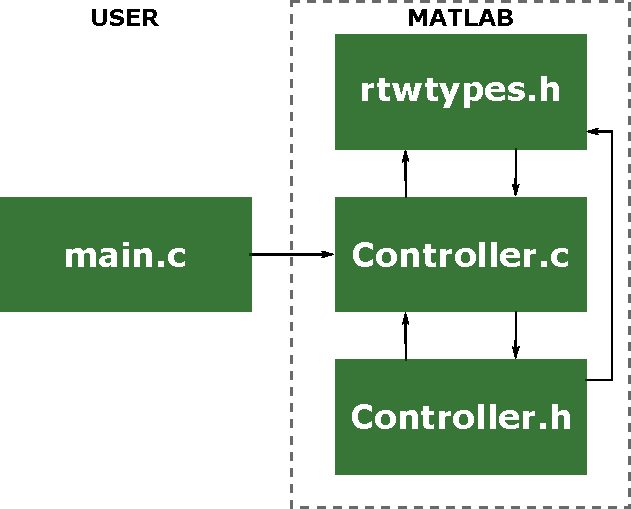
\includegraphics[width=0.6\linewidth]{img/rtw}
    \caption{Relationship of the generated files}
    \label{fig:rtw}
\end{figure}

The functions of the system are defined in the \textbf{controlsystem.c} and \textbf{controlsystem.h} files. The \textbf{rtwtypes.h} contains the unique type definitions of the code. The \textbf{ert\_main.c} is an exemplary main function that demonstrates the use of the others.

\subsection{Using the code}

The generated source code is functionally a perfect equivalent of the \verb!Simulink! model. The system can be initialized using the \emph{controlsystem\_initialize()} function. It sets the 0 time in the model and the outputs obtain their initial values. Communication with the system is only possible through a unique interface provided by the generated code. The inputs are handled by the \emph{controlsystem\_U struct}. It contains fields each corresponding to a system input, matching it's name and type. If the inputs are set, calling the \emph{controlsystem\_step()} function runs the model once, for the period of one time sample. The outputs are stored in a structure similar to the input storage, called \emph{controlsystem\_Y}.

\subsection{Deployment with FreeRTOS on STM32F4-Discovery Board}

As in many controlled processes, the timing of the controller program execution is crucial. Beside that it is also a time crucial task to process the I/O lines, convert the analog signals, and send status information to the supervisor computer over a wireless connection. It can be done with the integrated timer peripherals and with interrupt sequences, but the easiest way to handle a multi task problem like ours, is a \textbf{Real Time Operating System}. There are numerous implementation of these operating systems. We chose the FreeRTOS, which is a well known operating system in the industry, open-source, well documented and last but not least we have experience with it.

In our solution the FreeRTOS is responsible for the task scheduling, and provide a communication interface between the tasks. This way we can ensure that the sensors are read in the appropriate time, and the controller task will run in the specified time period. Also provides some useful tools to debug the application.
%Freertos mint Core mit csinál? (beszélget a hardverrel, szenzorokkal, aktuárotoknak küld beavatkozó jeleket)
%Miért jó? (gyors hozzáférés a szenzorokhoz, pontos ütemezés a controllernek)

Setting up the system is quite easy in this point. We only have to include the FreeRTOS source files into our project.\footnote{A detailed description is available for many processors in the FreeRTOS website: http://www.freertos.org/} The next step is to write some low level driver to read the sensors, and initialize the actuators so this way we can connect these to the control system. It is also necessary to set up the communication between the tasks, so we can read the state of the controller and the other tasks real time.
%Mit kellett csinálni, hogy működjön? (FreeRTOS-t feltenni rá (max 1 mondat, ebbe nem megyünk bele!), hardver jeleket kiolvasni C-vel, hogy oda tudjuk adni a controllernek, matlab-ot rákötni egy interrupt-ra)
%Még mit kell csinálni, hogy működjön?? Max 1-2 mondat már csak.